\documentclass[12pt, twoside]{article}
\usepackage[francais]{babel}
\usepackage[T1]{fontenc}
\usepackage[latin1]{inputenc}
\usepackage[left=7mm, right=7mm, top=5mm, bottom=5mm]{geometry}
\usepackage{float}
\usepackage{graphicx}
\usepackage{array}
\usepackage{multirow}
\usepackage{amsmath,amssymb,mathrsfs}
\usepackage{soul}
\pagestyle{empty}
\begin{document}

\section*{\center{Correction du devoir maison 5}}

\subsection*{Exercice 1}
\begin{tabular}{cc}
\begin{minipage}{7cm}
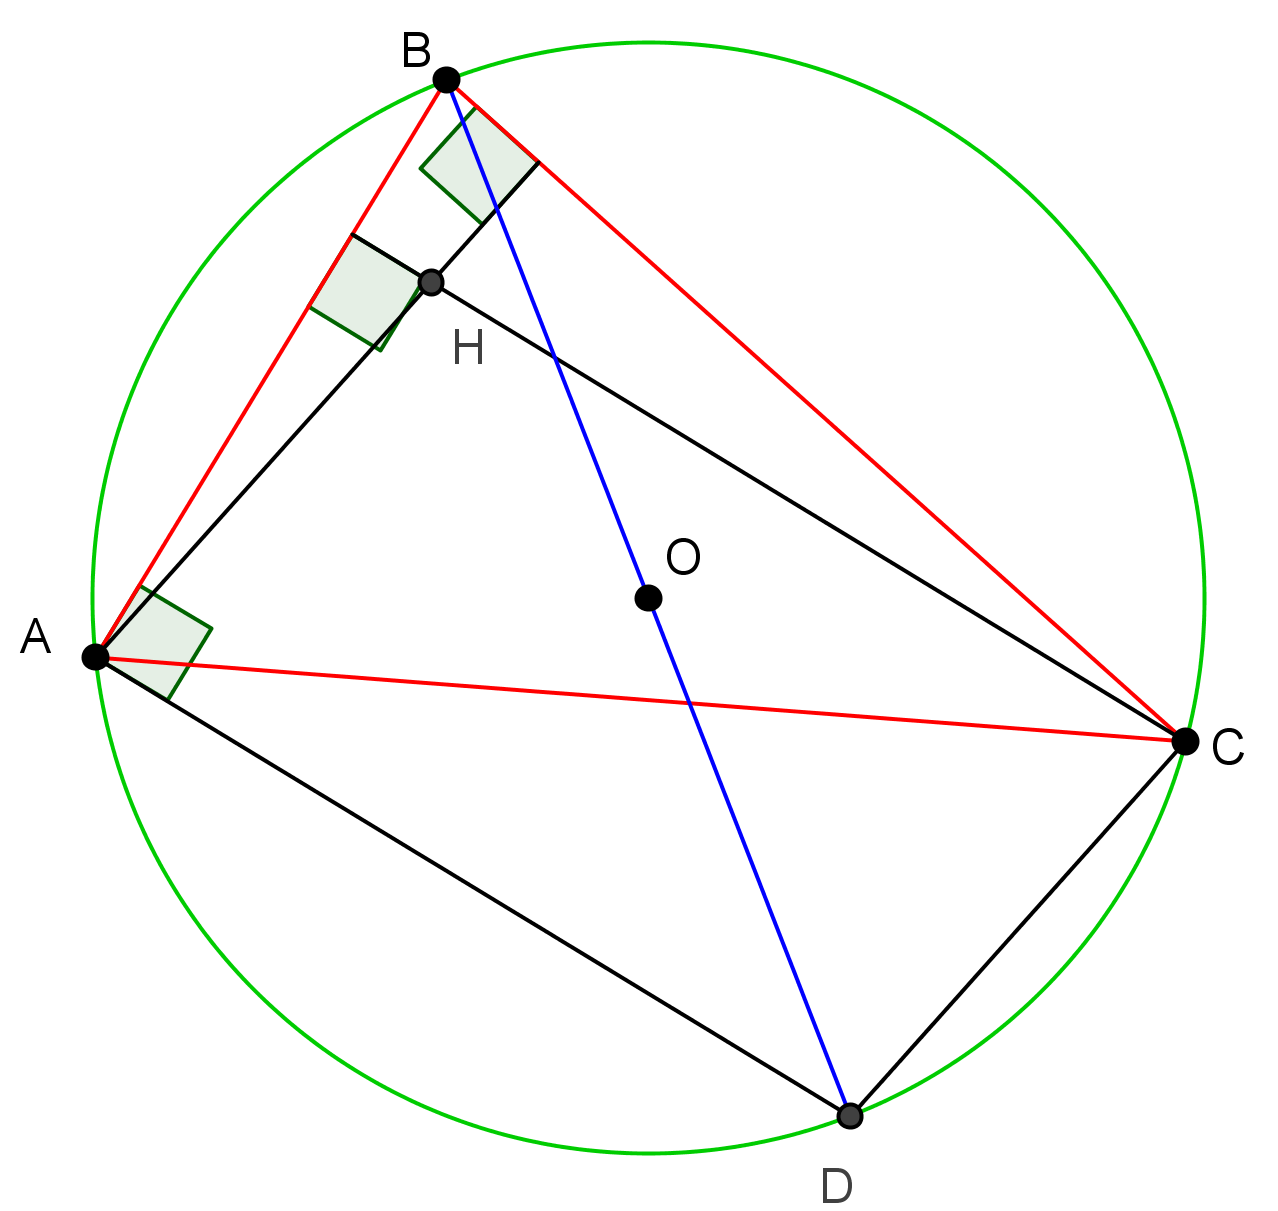
\includegraphics[width=7cm]{image/dm5.png}
\end{minipage}
&
\begin{minipage}{11cm}
\begin{enumerate}
  \item $ABD$ est un triangle rectangle d'hypot�nuse $[BD]$. $\mathcal{C}$ est
  le cercle circonscrit du triangle $ABD$. Donc $[BD]$ est un diam�tre de
  $\mathcal{C}$.
  \item $[BD]$ est un diam�tre de $\mathcal{C}$, $C$ est un point de
  $\mathcal{C}$ donc le triangle $BCD$ est rectangle en $C$.
  \item $(CH)$ et$ (AB)$ sont perpendiculaires car $[CH]$ est la hauteur issue
  de $C$ du triangle $ABC$. $(AD)$ et $(AB)$ sont perpendiculaires par
  hypoth�se, donc $(CH)$ et $(AD)$ sont parall�eles.
  
  \enskip
  
  
  $(AH)$ et $(BC)$ sont perpendiculaires car $[AH]$ est la hauteur issue
  de $A$ du triangle $ABC$. D'apr�s la question pr�c�dente, $(BC)$ et $(CD)$
  sont perpendiculaires donc les droites $(AH)$ et $(CD)$ sont parall�les.
\end{enumerate}

\end{minipage}
\end{tabular}

\enskip

Les c�t�s oppos�s du quadrilat�re $AHCD$ sont deux � deux parall�les donc
$AHCD$ est un parall�logramme.

\subsection*{Exercice 3}

\begin{tabular}{cc}
\begin{minipage}{8cm}
$(x-3)^{2}-36=0 $\\
$(x-3)^{2}-6^{2}=0$\\
$(x-3-6)(x-3+6)=0$\\
$(x+3)(x-9)=0$\\
donc $x+3=0$ ou $x-9=0$\\
les solutions sont $x=-3$ et $x=9$.
\end{minipage}
& 
\begin{minipage}{8cm}
$(2x-1)(x-6)-3(1-2x)+1=2x$\\
$(2x-1)(x-6)-3 \times (-1)(2x-1)+1-2x=0$\\
$(2x-1)(x-6)+3(2x-1)+(-1) \times (2x-1)=0$\\
$(2x-1)[(x-6)+3-1]=0$\\
$(2x-1)(x-4)=0$\\
donx $2x-1=0$ ou $x-4=0$\\
les solutions sont $x=\dfrac{1}{2}$ et $x=4$.
\end{minipage}
\end{tabular}
\medskip

$\dfrac{(7x+2)(x-1)}{3x+5}=0$


Recherche de la valeur interdite: $3x+5=0$ donc $x=-\dfrac{5}{3}$\\
$(7x+2)(x-1)=0$ donc $7x+2=0$ ou $x-1=0$.

$x=-\dfrac{2}{7}$ ou $x=1$.
$-\dfrac{5}{3} \neq -\dfrac{2}{7}$ et $-\dfrac{5}{3} \neq 1$ donc les solutions
sont $-\dfrac{2}{7}$ et $1$.
 
\subsection*{Exercice 4}

\begin{tabular}{cc}
\begin{minipage}{4cm}
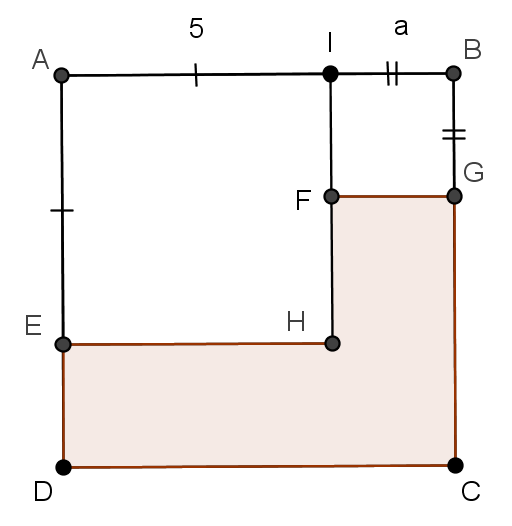
\includegraphics[width=4cm]{image/ex.png}
\end{minipage}
&
\begin{minipage}{15cm}
$Aire(ABCD) = Aire(FGCDEH)- Aire(AIHE)-Aire(IBGF)$


 \qquad \qquad \quad \quad $=(5+a)^{2}-5^{2}-a^{2}=10a$.\\
 De plus par hypoth�se, $Aire(ABCD)=36$ donc $10a=36$ et $a=3,6$.
 On en d�duit le p�rim�tre de $ABCD$: $4 \times (5+3,6)=34,4$.
\end{minipage}
\end{tabular}


\end{document}
